%#! platex %f && dvipdfmx -d 5 sample221227report
%
% \documentclass[a4paper,11pt,dvipdfmx]{ujarticle}   % uplatex の場合
\documentclass[a4paper,11pt,dvipdfmx]{jarticle}  % platex の場合

\usepackage[dvips,usenames]{color} 
\usepackage{graphicx}
\usepackage{fancyhdr}
\usepackage{bm}  % for bmdefine
\usepackage{amsmath} % bmatrix, pmatrix
\topmargin = -5mm
\oddsidemargin = 5mm
\textwidth = 152mm
\textheight = 240mm
% \pagestyle{empty}
\pagestyle{fancyplain}
\renewcommand{\footrulewidth}{0pt}
\renewcommand{\headrulewidth}{0pt}
\bmdefine{\bx}{w}
\bmdefine{\bx}{x}
\bmdefine{\by}{y}
\bmdefine{\be}{e}
\everymath{\displaystyle}

\begin{document}
\lhead{\small 情報通信工学プログラム}
\rhead{\small 2022年12月27日\\宮崎イチロー}
% \cfoot{}


\centerline{\Large\gt \LaTeX を使ったレポート作成}      
\vskip 5mm
\centerline{\Large\gt 60277777 宮崎 イチロー}


\section{はじめに} 
実験したことはレポートに書いておこう.
分かりやすく簡潔に書こう.
どこまで
「分かりやすく」書けばいいかというと,
1年前の自分が読んで理解できればよい.
簡潔とは言っても,単に短いだけではだめで少なくとも
\begin{enumerate}
\item 何を実験したのか,一つ一つの手順.
\item 得られた結果(図)の説明(横軸,縦軸,プロットしている線,点の意味など)
\item 考察,自分の意見,感想
\end{enumerate}
が必要.
図を張り付けただけで説明がない場合,0点をつけられても仕方がない.
%
% このソースファイルを読んで,いろいろ数字を変更し,使い方をマスターしよう.
%
詳しい \LaTeX の使い方については,
{\tt Google} で 「{\tt latex},レポート作成」などと検索
すれば親切なページが発見できる.
「教えてもらっていない」なんていう人は $\cdots$
($\Longrightarrow$ 卒業できない.さようなら).


\section{いろいろなことができる}
\subsection{図はどうするか}
{\tt gnuplot} などで,図を作成した場合,
画面に表示している図をそのまま取り込むのではなく,
直接 {\tt pdf} などベクトル形式の情報が含まれたファイルを生成するようにしておく.
\begin{figure}[h]
\begin{center}
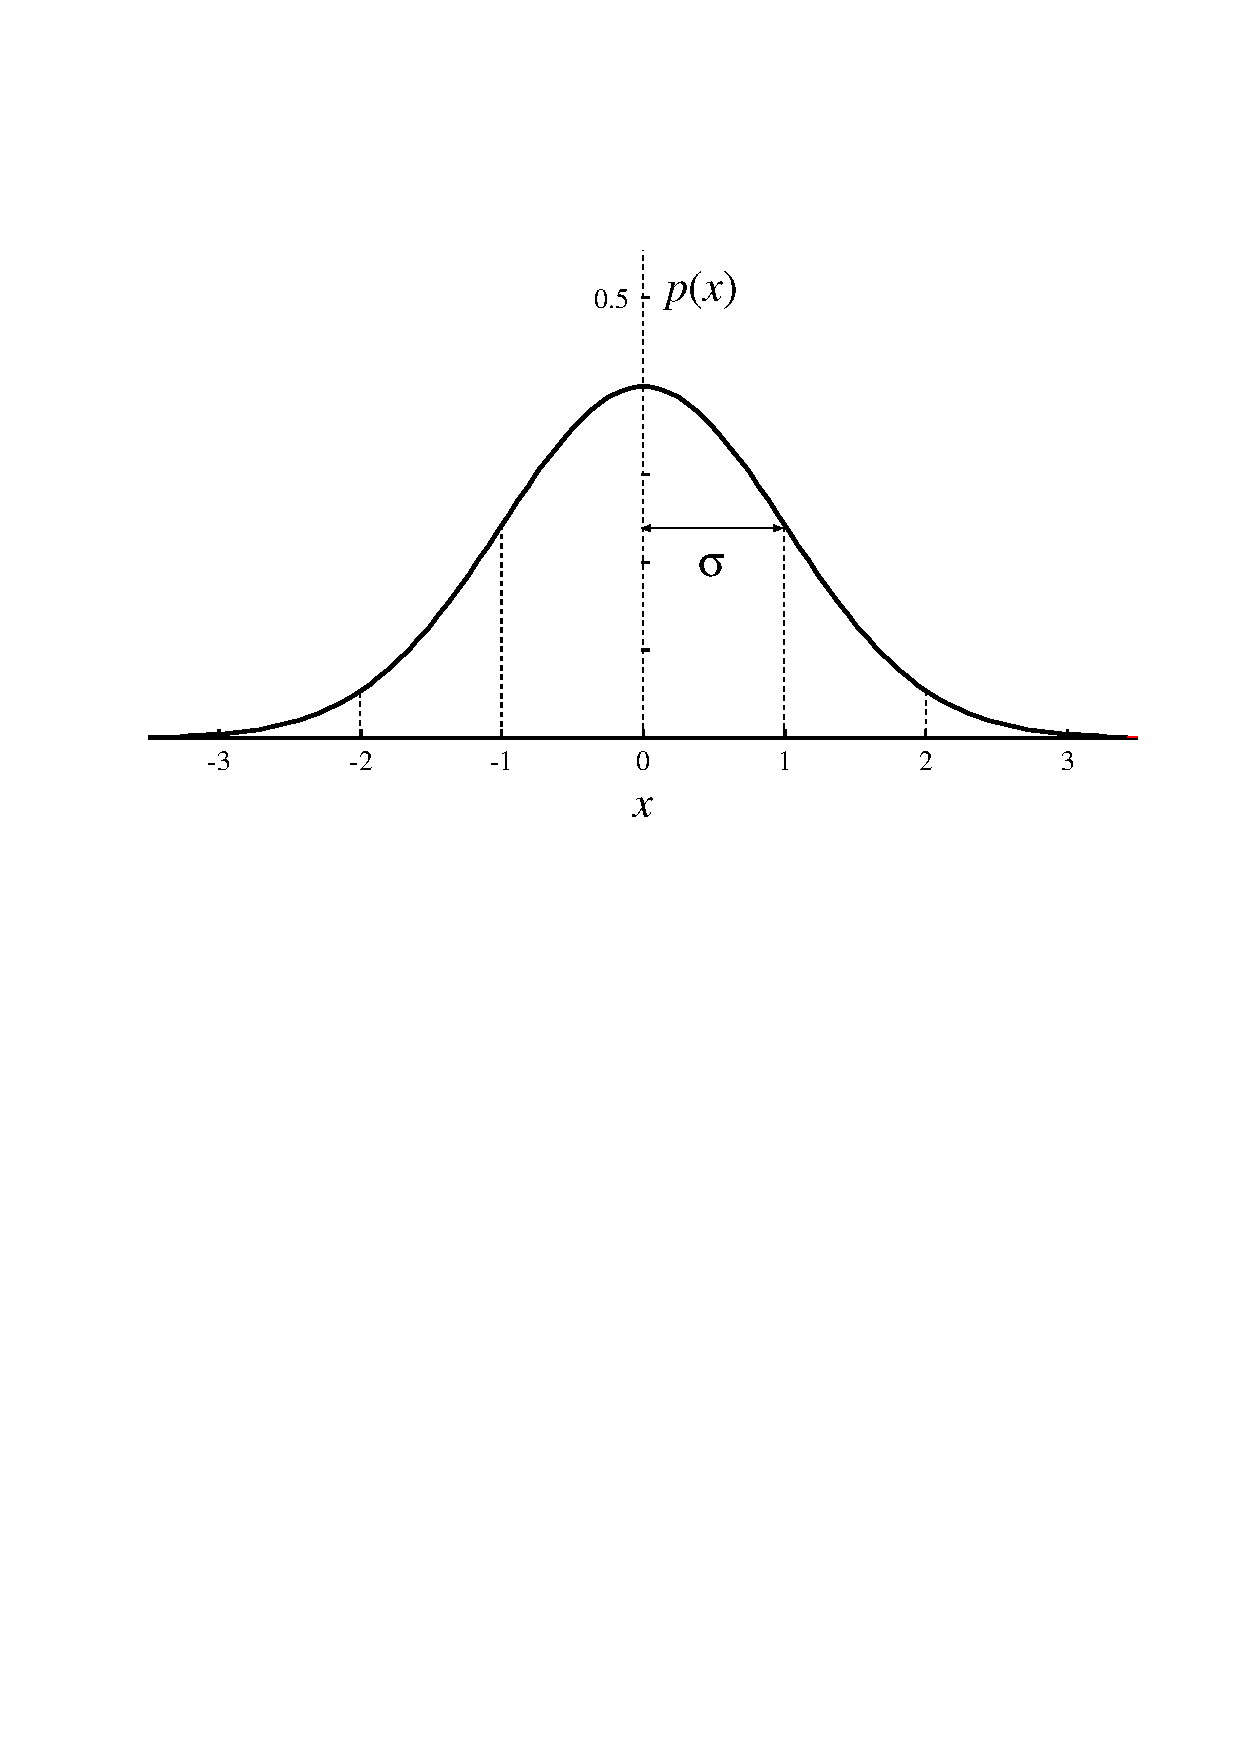
\includegraphics[width=.4\linewidth]{gauss001.pdf}
\hspace*{2mm}
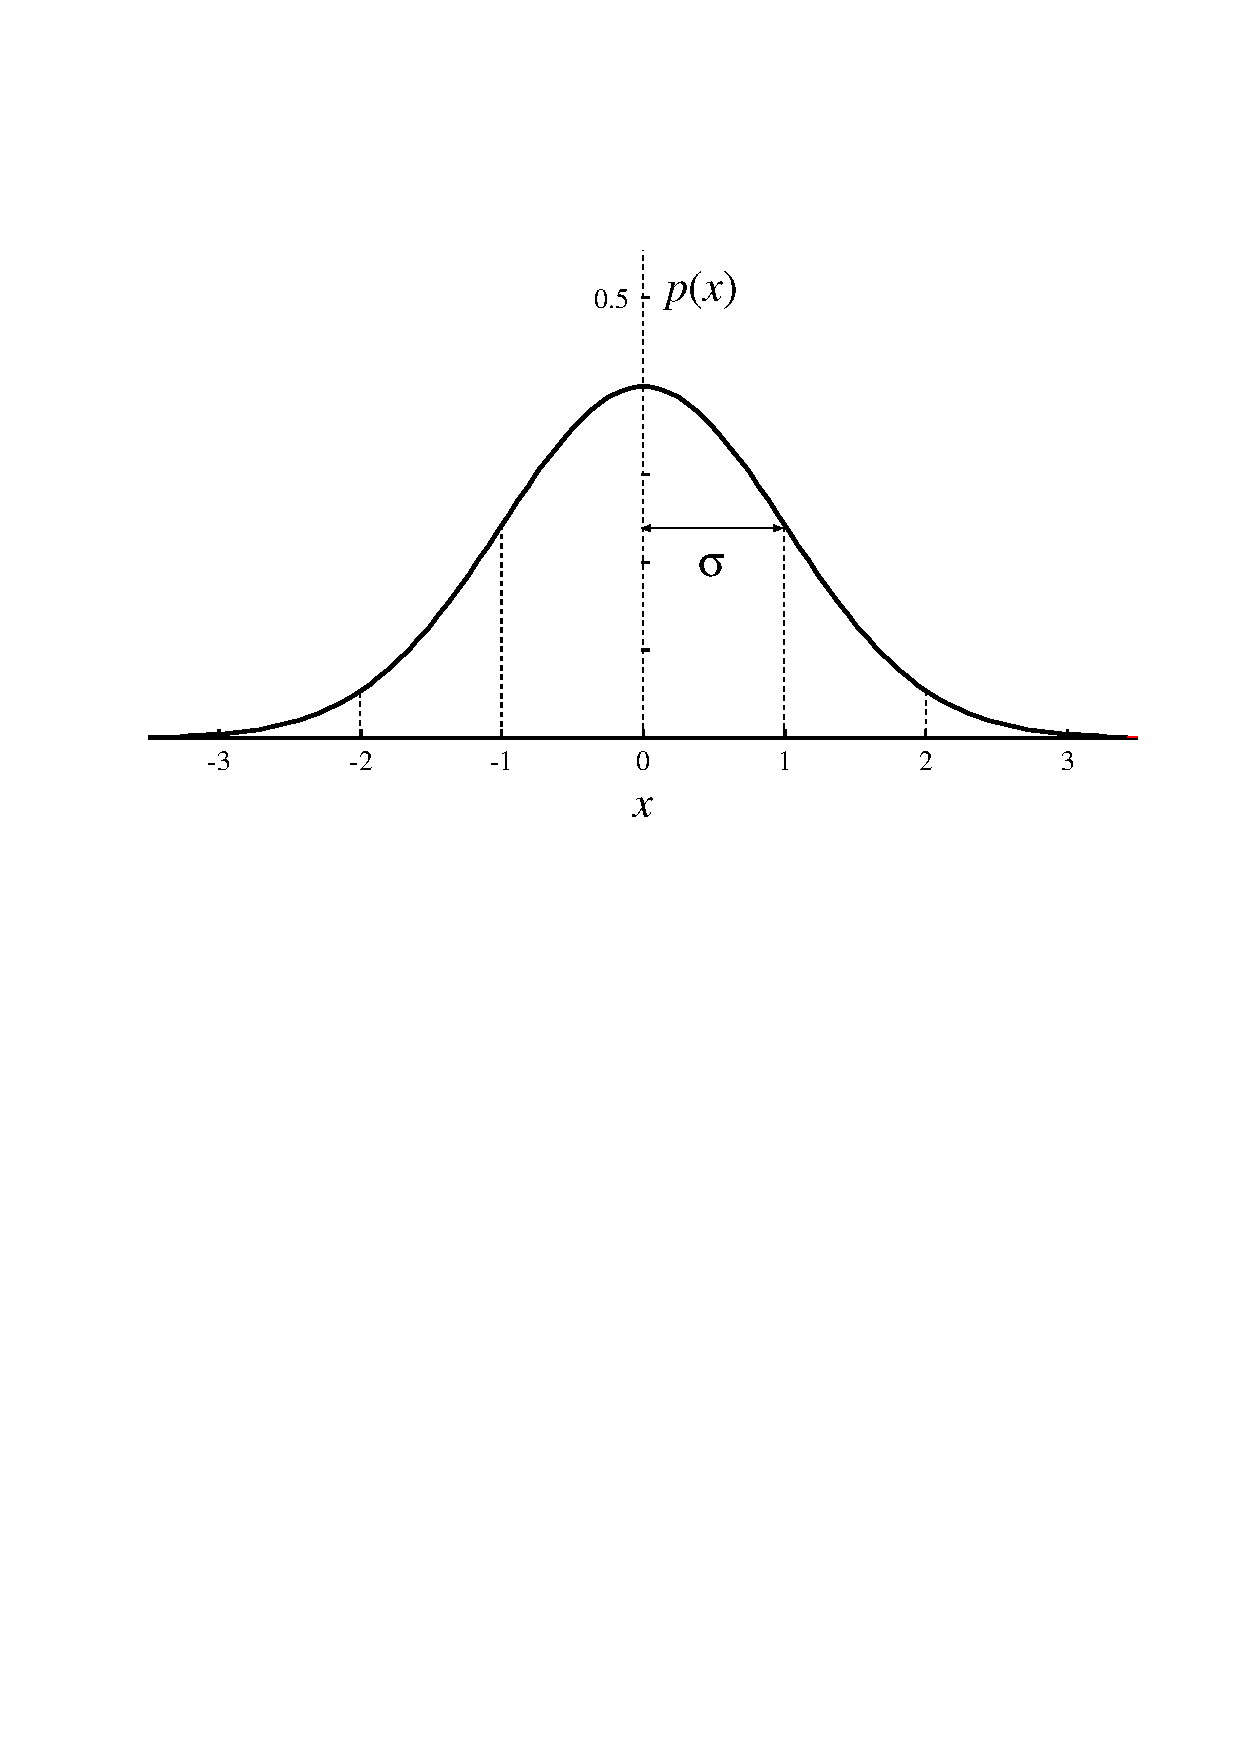
\includegraphics[width=.4\linewidth]{gauss001.pdf}
\caption{平均 $0$,分散 $1$ の正規分布の確率密度関数}
\end{center}
\end{figure}


\subsection{数式は?}
普通の文章中では $ y = \sin (x)$. 式番号が必要なら
\begin{eqnarray}
a &= & \int_{-\infty}^{10}  \frac{x^2+3 \pi}{4\theta} dx \\
b & = & a + 3 \\
\bx & = & (100 \gamma, 1) \nonumber 
\end{eqnarray}

%
% これはコメント
%
%
%

\newpage


\subsection{疑問点の整理の仕方の一例}
\centerline{\Large\gt 疑問点の整理}
\vspace{2mm}
\noindent
工学と固有値\\
\begin{center}
\begin{tabular}{|c|p{5zw}|p{15zw}|p{15zw}|} \hline
頁 & 箇所 & 内容 & 疑問点など \\ \hline
12 & 
右の4行目付近
& 
$ A \be_1 = \lambda_1 \be_1 $ で,
$A$ は$\be_1$ に対しては単に数$\lambda_1$を掛けるだけの働き
&
行列をかけなくても$\lambda_1$
をかけたらいいのはなぜなのか.
\\ \hline
%
%
15  &
右側後半
&
固有値 $\lambda_1=6, \lambda_2=1$のそれぞれに対応する固有ベクトルを規格化してそれらを並べた行列である$P$と$P^\top$を求めている部分.
これらの $ P $ と $ P^\top $を比較して
$P$は直交行列になるという記載の後に
『$\be_1$と$\be_2$が直交していたので,$|\be_1 |=1, |\be_2|=1$に規格化すればよい』と記載されている. &
規格化するタイミングと規格化する必要性が理解できない.
$\be_1$ と $\be_2$ を規格化して$P$を求めた結果,
$P$ が直交行列になったという流れなのか,
そもそも $\be_1$と$\be_2$が直交していたのだからでそれらを並べた$P$は直交行列であるという理屈ならば規格化する必要はないのではないかと考える.\\ \hline
& & & \\ \hline
& & & \\ \hline
& & & \\ \hline
\end{tabular}

\end{center}


\lhead{}  % 2ページめ以降には,日付,名前を表示しない
\rhead{}


\begin{thebibliography}{99}  %   文献数が10未満の時 {9}

\bibitem{amari91a}
甘利 俊一,``ニューロ多様体の情報幾何学,'' 
数理科学, no. 340, pp. 61--65, Oct, 1991.

\end{thebibliography}



\section*{付録}

\begin{figure}[htbp]
 \begin{minipage}{0.5\hsize}
  \begin{center}
   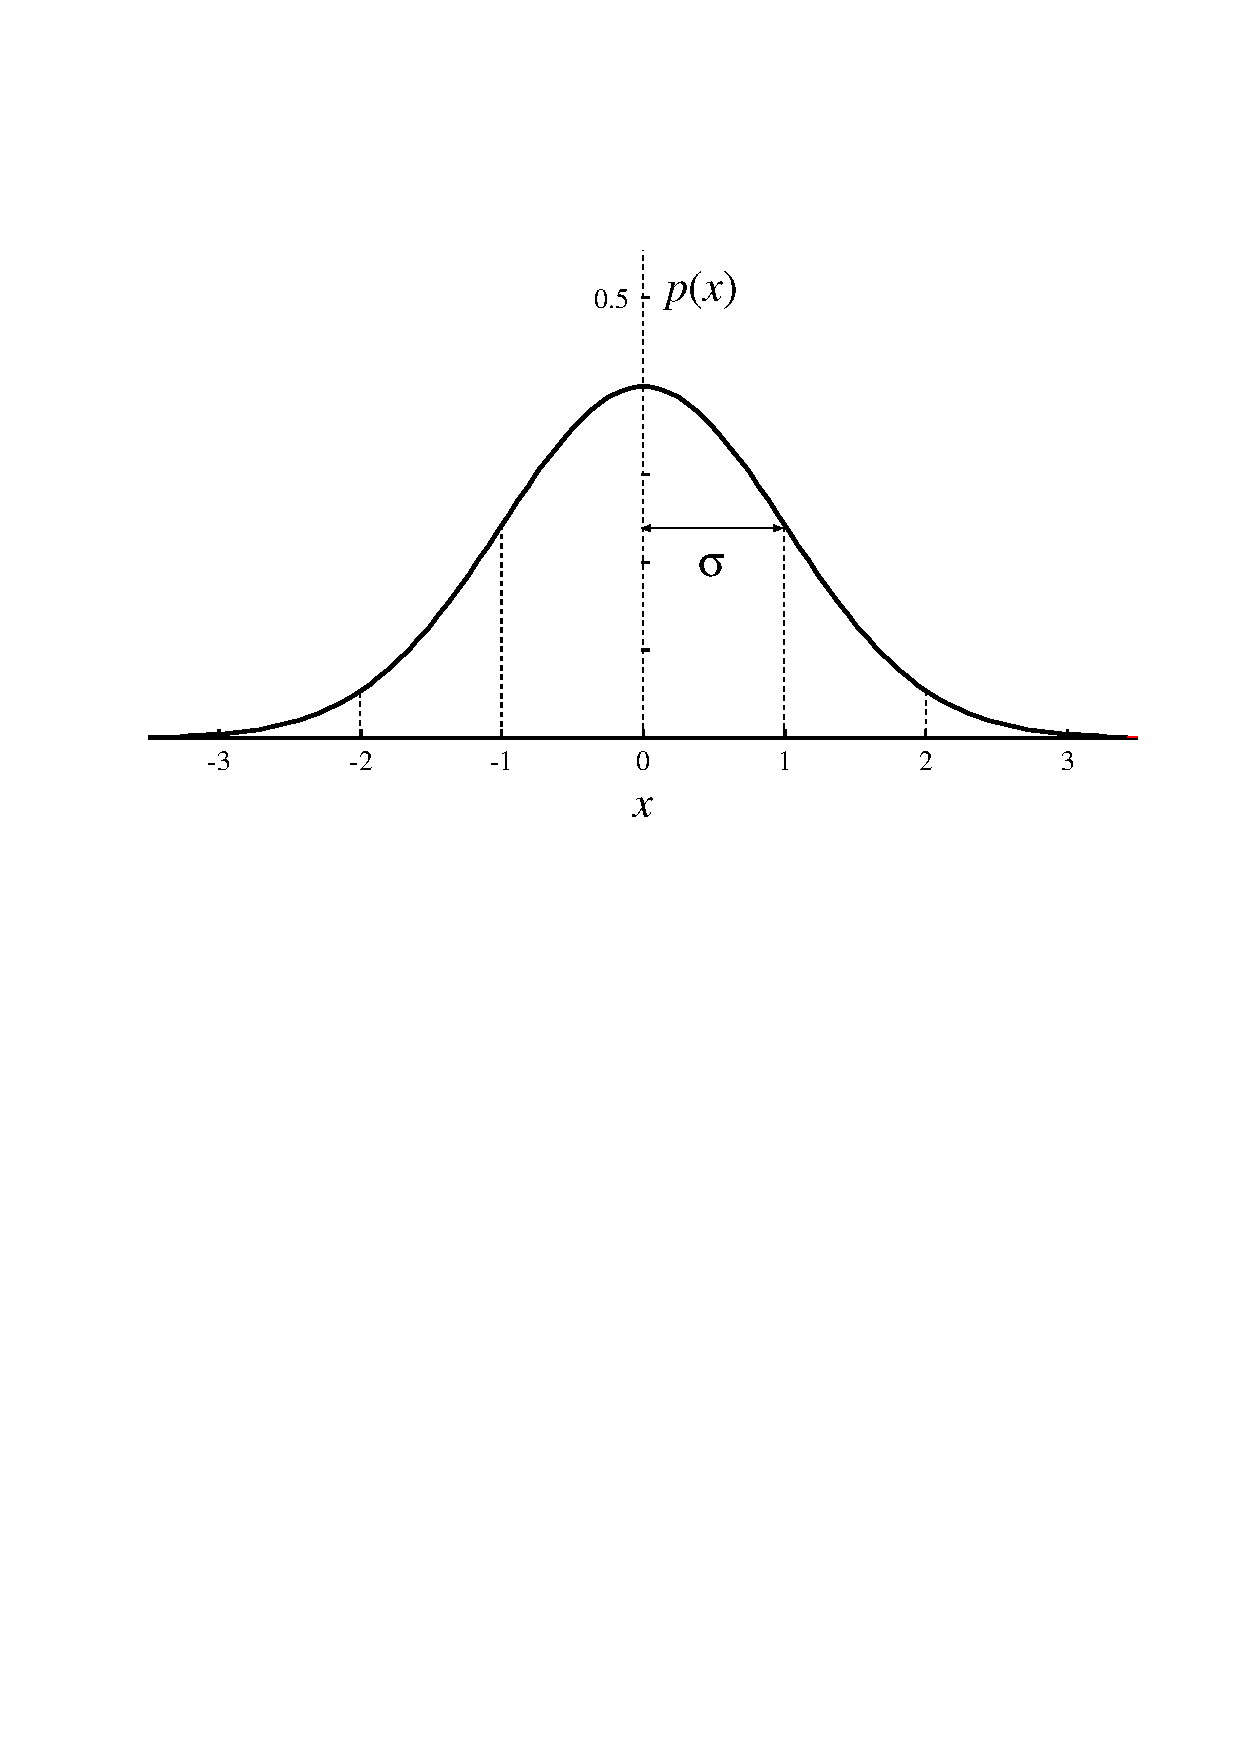
\includegraphics[width=70mm]{gauss001.pdf}
  \end{center}
  \caption{1つめの図}
  \label{fig:one}
 \end{minipage}
 \begin{minipage}{0.5\hsize}
  \begin{center}
   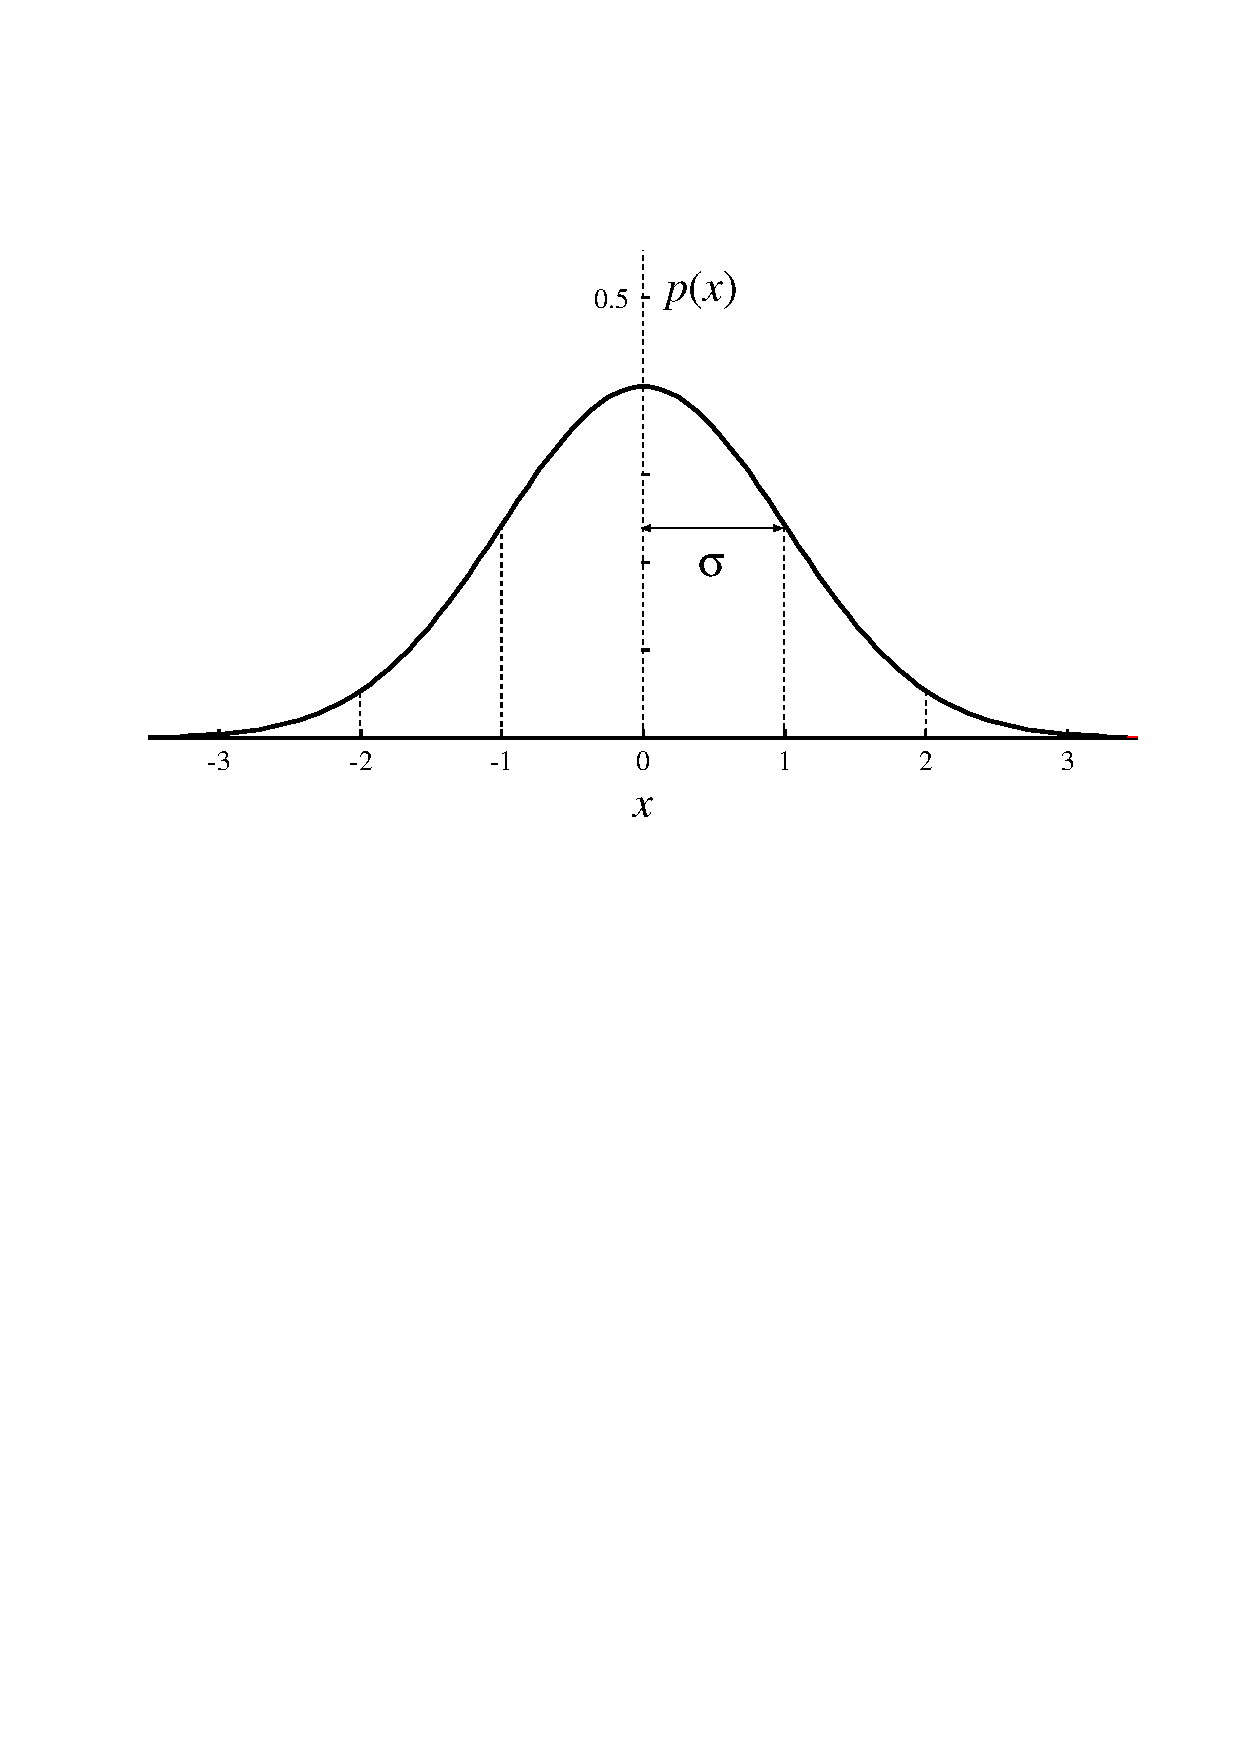
\includegraphics[width=70mm]{gauss001.pdf}
  \end{center}
  \caption{2つめの図}
  \label{fig:two}
 \end{minipage}
\end{figure}


\begin{figure}[htbp]
 \begin{minipage}{0.33\hsize}
  \begin{center}
   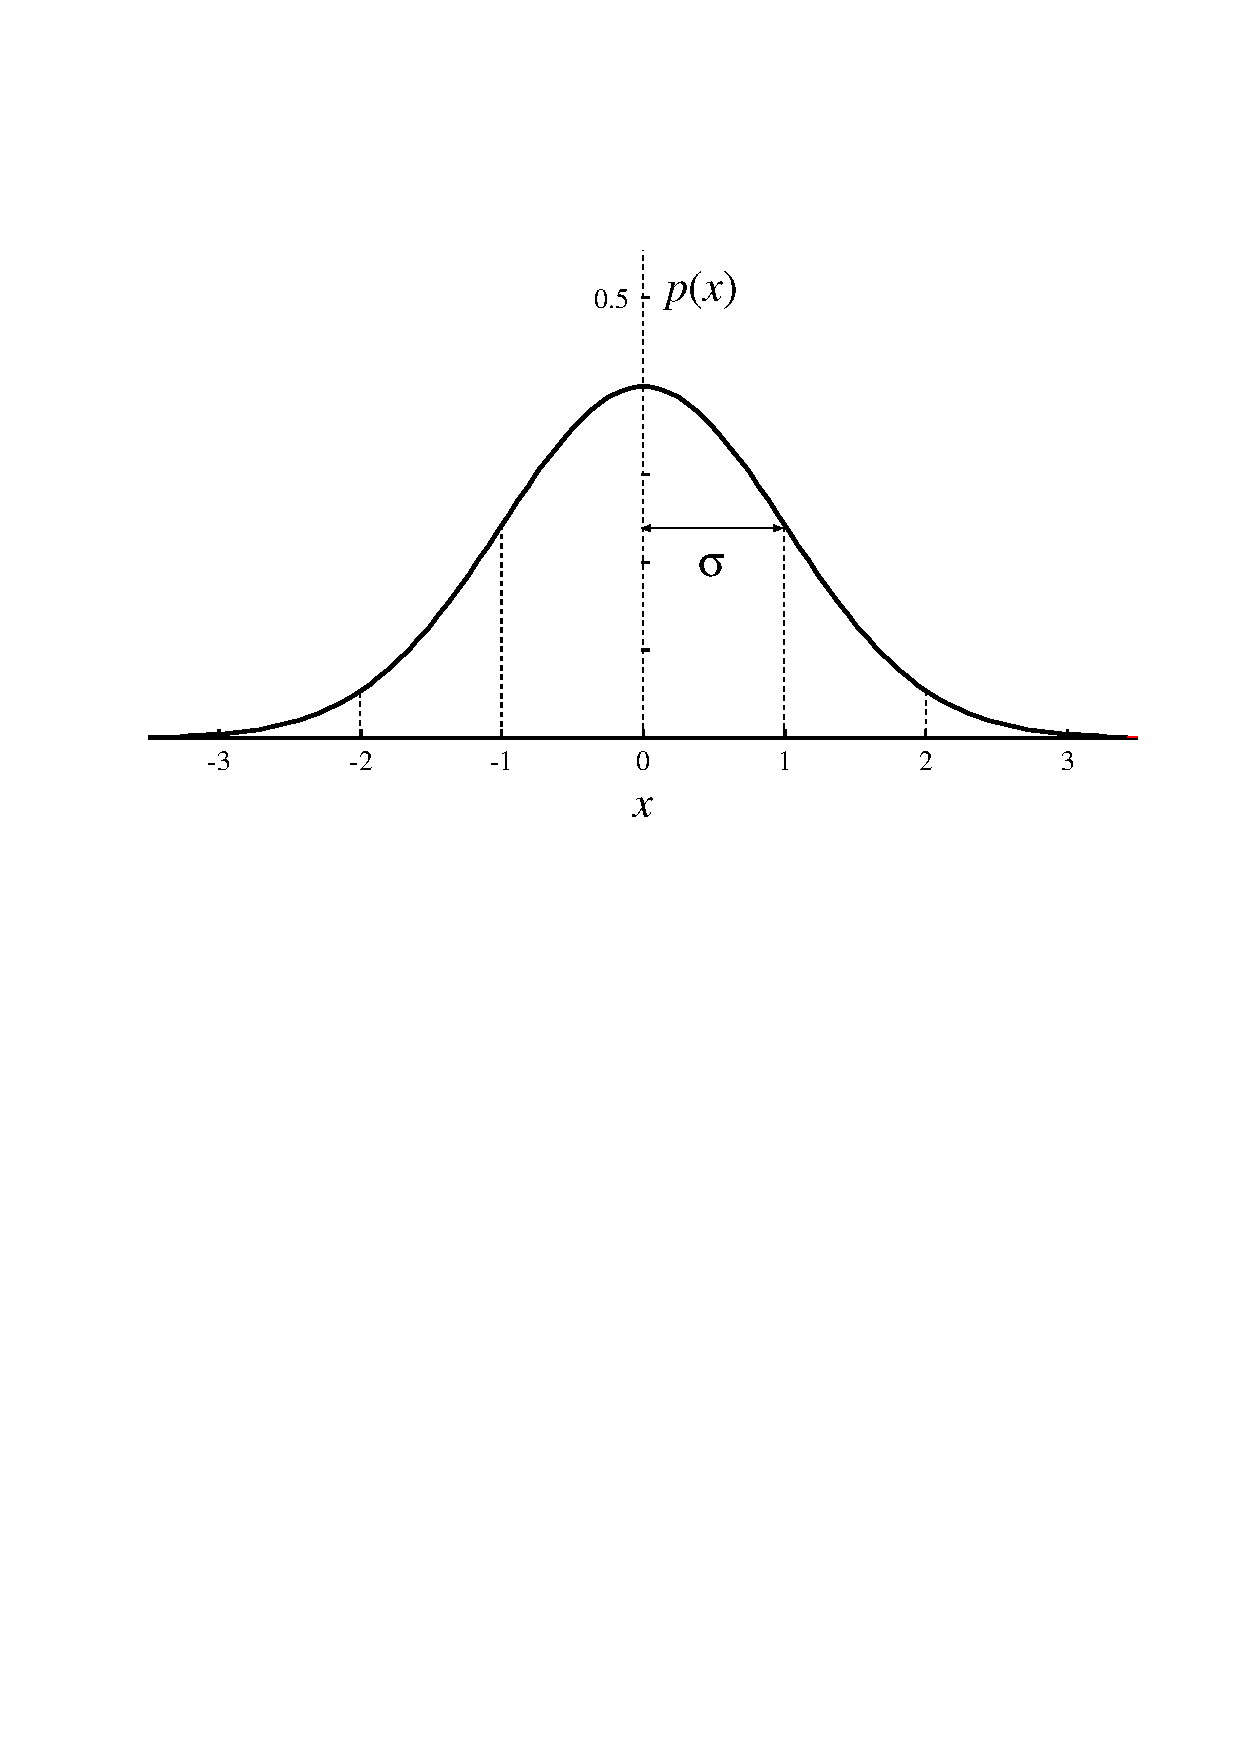
\includegraphics[width=40mm]{gauss001.pdf}
  \end{center}
  \caption{3つめの図}
  \label{fig:three}
 \end{minipage}
 \begin{minipage}{0.33\hsize}
 \begin{center}
  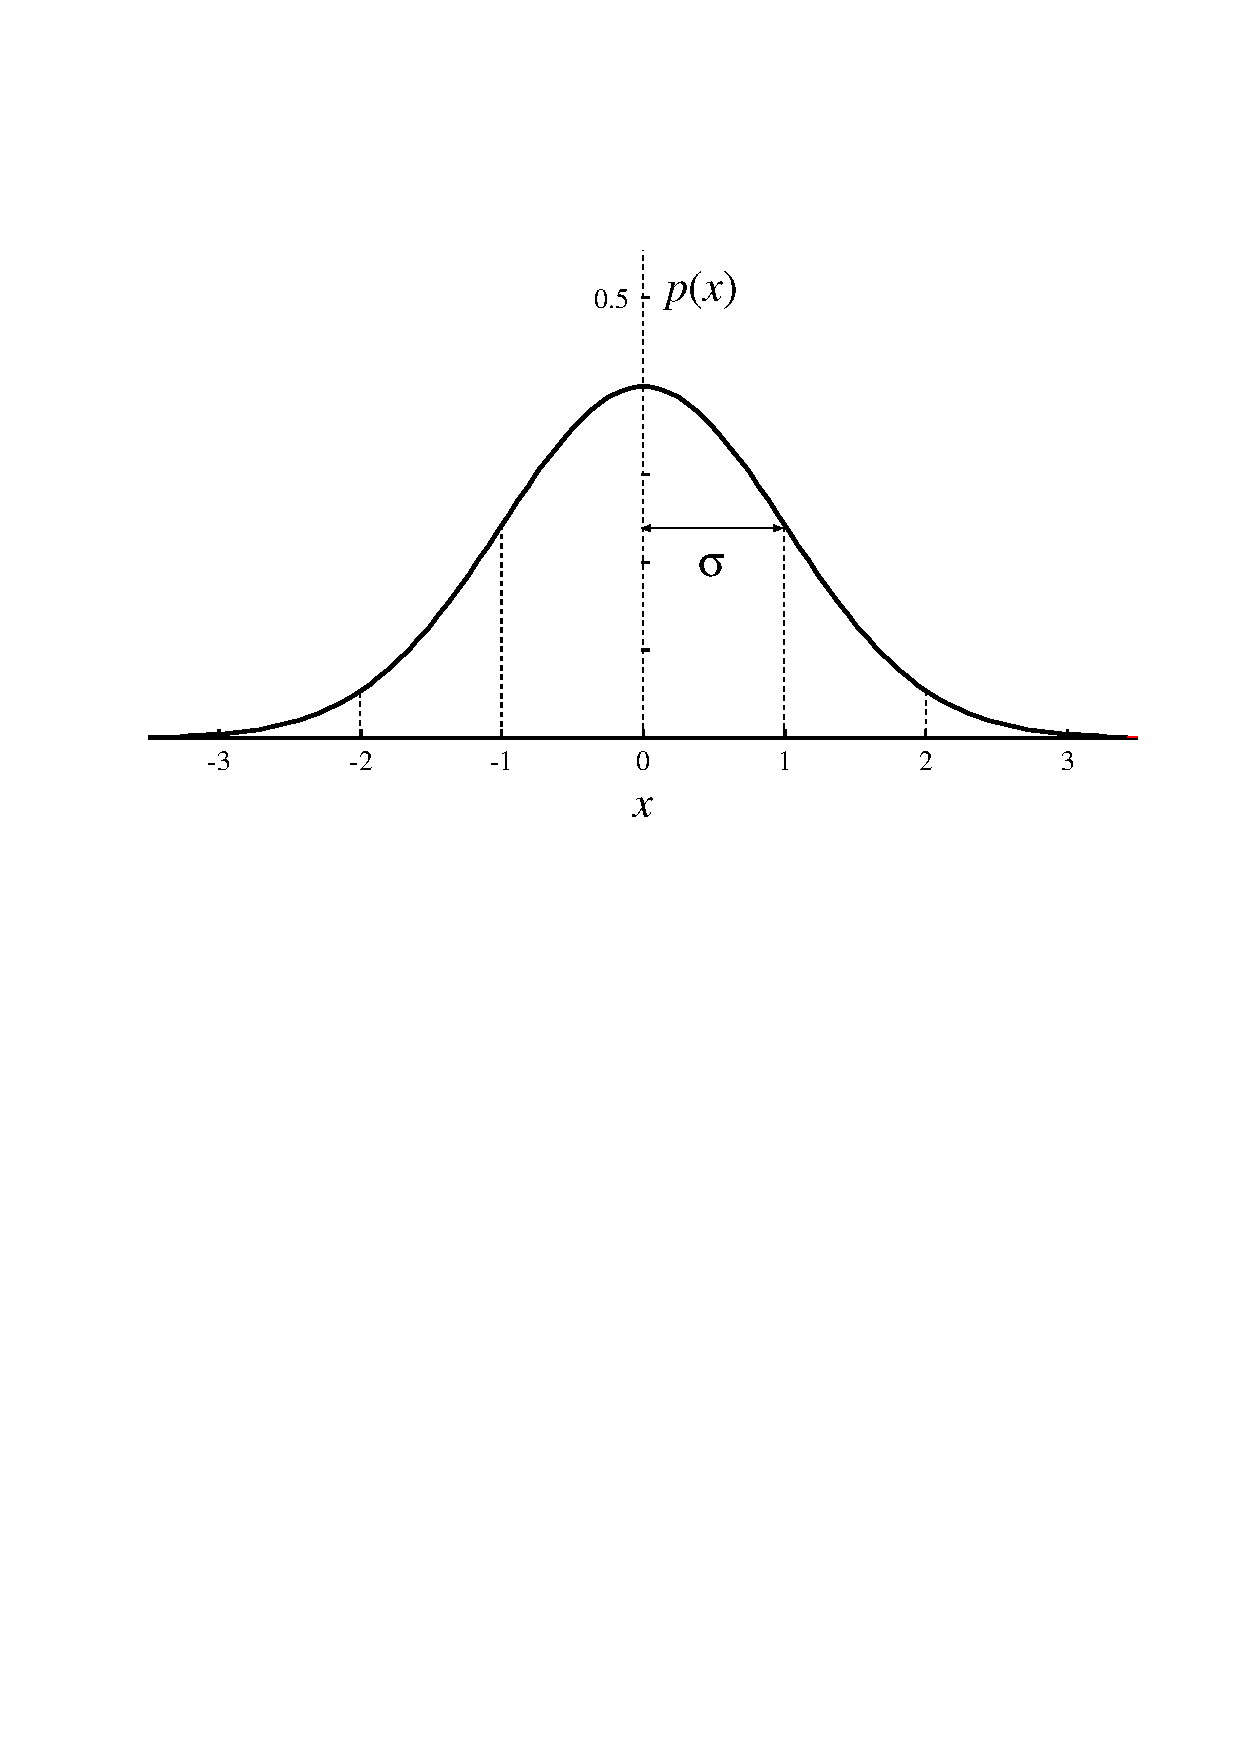
\includegraphics[width=40mm]{gauss001.pdf}
 \end{center}
  \caption{4つめの図}
  \label{fig:four}
 \end{minipage}
 \begin{minipage}{0.33\hsize}
 \begin{center}
  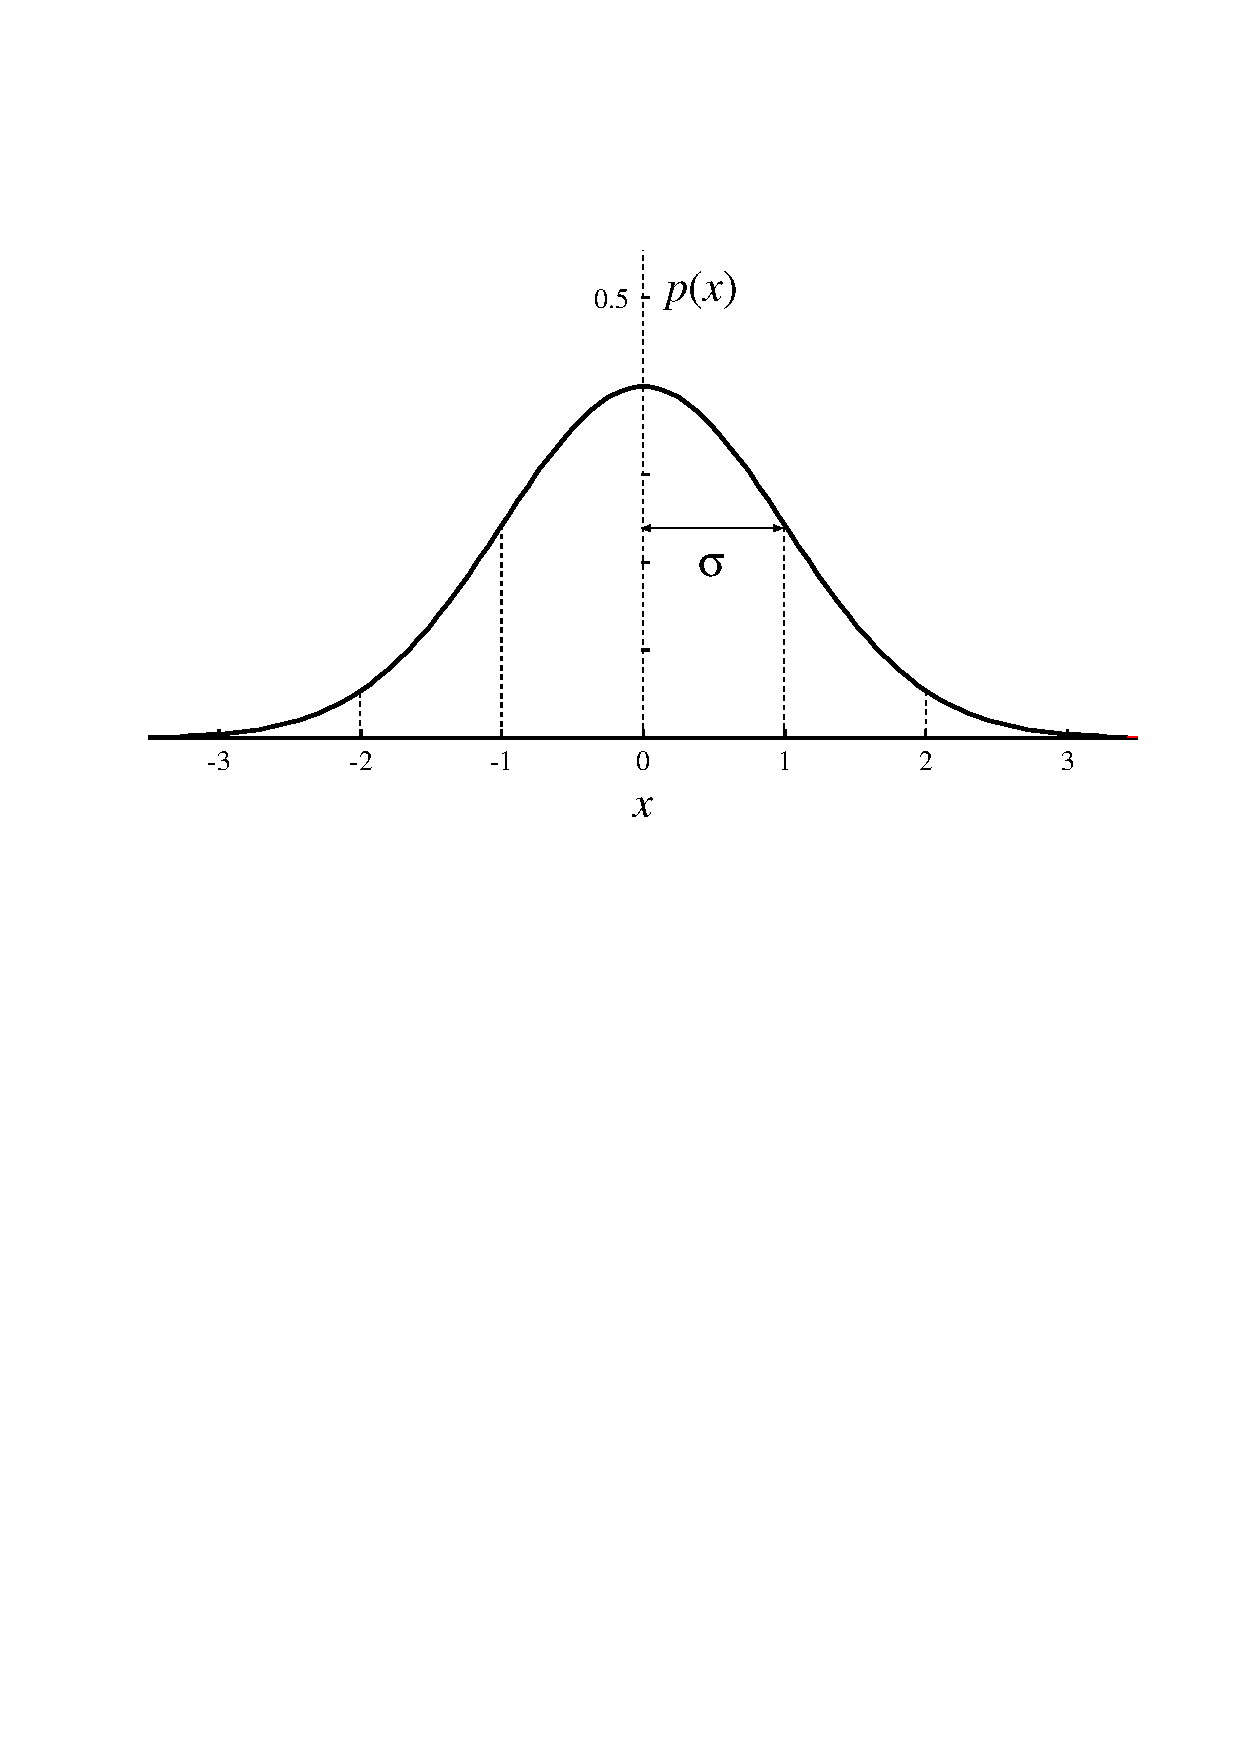
\includegraphics[width=40mm]{gauss001.pdf}
 \end{center}
  \caption{5つめの図}
  \label{fig:five}
 \end{minipage}
\end{figure}


図\ref{fig:three} は左下の図です.

\lhead{}
\rhead{}


\begin{eqnarray}
\frac{dx}{dt}   & = &  - 3x \\
\frac{dx}{dt}  +2x  & = & 2t + 5 \\
x' + 2tx & = & 4t  \\
x' & = & \mathrm{e}^{-t^2} -2tx \\
x' + x & = &  \mathrm{e}^{-t} \\
x' - (\sin t) x  & = &  \sin (2t) \\
x' + x  & = &  x^2 \mathrm{e}^t \\
x' - tx   & = &  - x^3 \mathrm{e}^{-t^2}  \\
\tau \frac{dx}{dt} & = &   -x + 1 \\
\tau \frac{dx}{dt} & = &   -x + \cos t 
\end{eqnarray}

\vskip 1mm

\begin{eqnarray}
\int_1^{x} \frac{1}{x}dx   & = &  - 3 \int_0^t dt \\
\dot {\bm{x}} & = & A \bm{x} \\
\mathrm{e}^{A} & = & \sum_{k=0}^\infty \frac{A^k}{k!}
\end{eqnarray}

\begin{eqnarray}
\begin{pmatrix}
1 & 1 & 1 \\
2 & 1 & 2
\end{pmatrix}
\begin{pmatrix}
x \\
y \\
z
\end{pmatrix} 
& = &
\begin{pmatrix}
3 \\
2
\end{pmatrix}
\\
\begin{bmatrix}
1 & 1 & 1 \\
2 & 1 & 2
\end{bmatrix}
\begin{bmatrix}
x \\
y \\
z
\end{bmatrix} 
& = &
\begin{bmatrix}
3 \\
2
\end{bmatrix}
\\
A \bm{x}  & = & \bm{y}
\\
x_i & = & f \left ( \sum_{j=1}^n w_{ij}  x_j \right )
\\
% 条件付きの式
p(t) & = & \left\{ \begin{array}{ll}
 1 &  (|t| \geq 1 ) \\
 0 &  (|t| > 1 )
 \end{array}
 \right. 
\\
% \text は数式モード内でローマン体にしたい文字に対して有効
\bx_{\text{MAP}} & = &   
\mathop{\text{argmax}}_{\bx} 
p(\bx|\by_{\text{obs}} ) 
\end{eqnarray}


\end{document}


